\chapter{Framework MVC propio\label{extra:framework_mvc_propio}}

En este apéndice se explican los distintos componentes del \gls{framework} propio desarrollado, del que hace uso la interfaz web. 
Lenguajes (php), javascript, html, css
apache

TODO: [Introducción], Imagen, módulo CORE
  {Visión global}
TODO: Decidir si se ponen aquí lo de las traducciones

\section{Modelo Vista Controlador\label{extra:mvc:mvc}}

TODO: Modelo Vista Controlador, interacción entre componentes, división en módulos,
clases abstractas

\begin{figure}[!htp]
  \centering
  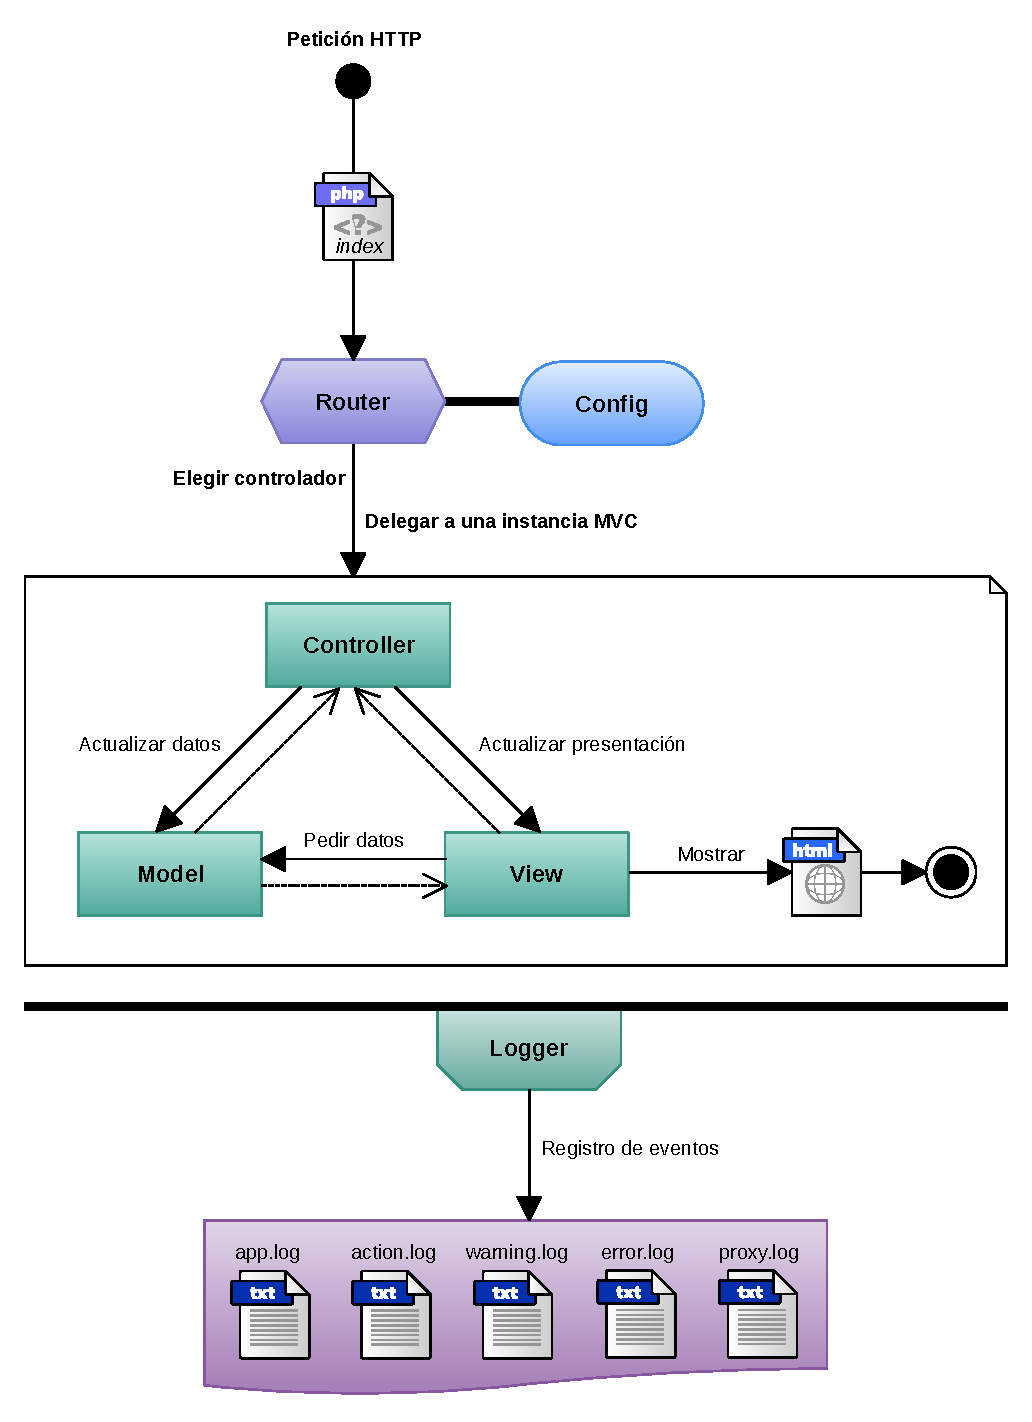
\includegraphics[width=\textwidth,clip=true]{graphics/framework}
  \caption{Arquitectura del \gls{framework} propio.}
  \label{fig:framework}
\end{figure}

\section{Manejo de rutas\label{extra:mvc:router}}

/módulo/método/param1/param2
TODO: Router, redireccionamiento, urls rest, parámetros, proxy, htaccess

\section{Redireccionamiento de peticiones a servicio web\label{extra:mvc:proxy}}

Proxy, por qué es necesario, AJAX, paso de parámetros
facilitar seguridad, red local

\begin{figure}[!htp]
  \centering
  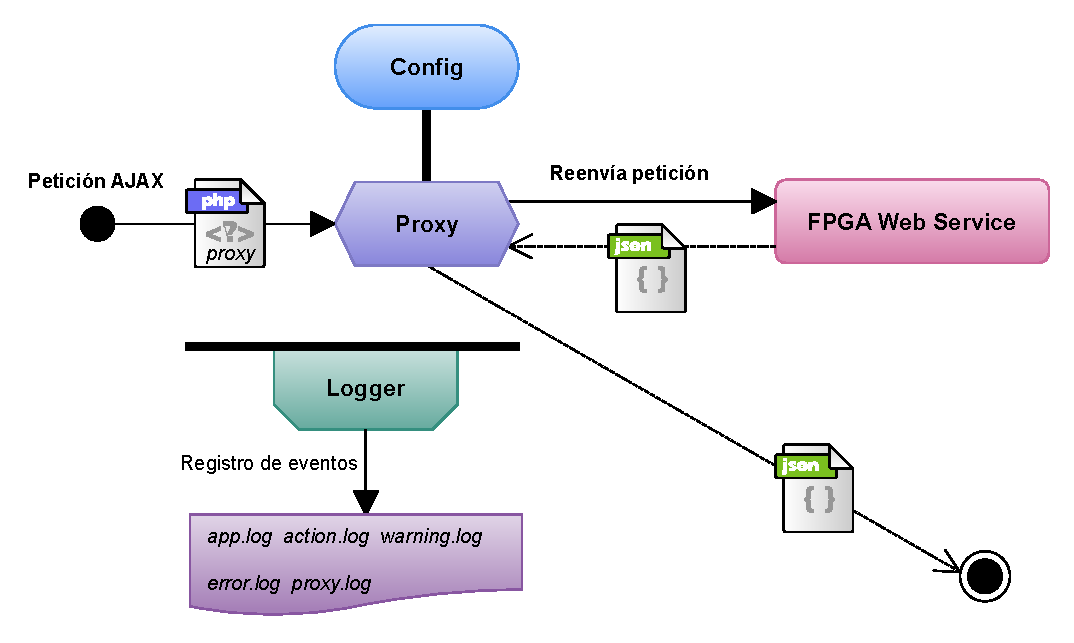
\includegraphics[width=0.6\textwidth,clip=true]{graphics/proxy}
  \caption{Arquitectura del proxy propio.}
  \label{fig:proxy}
\end{figure}

\section{Internacionalización de la interfaz\label{extra:mvc:i18n}}

Este \gls{framework} facilita la traducción de la aplicación a distintos idiomas mediante la librería \textit{gettext} \cite{gettext} para \gls{PHP}. Esta librería proporciona funciones (\textit{\_} y \textit{gettext}) que reciben cadenas de texto y devuelven su equivalente en el idioma de la aplicación seleccionado, consultando un archivo previamente creado (catálogo) que contiene cadenas de texto originales y su traducción.

Es necesario un catálogo por cada idioma que se quiera añadir a la aplicación. Los catálogos se almacenan en la carpeta del proyecto \texttt{./locale/}. Para crear y gestionar los catálogos es recomendable utilizar la herramienta \textit{Poedit} \cite{poedit}, que permite editarlos con una interfaz gráfica. Para obtener las cadenas de texto que se necesitan traducir, se escanean todos archivos del proyecto en busca de las palabras clave, y se añaden las cadenas de texto al catálogo para su traducción por parte del desarrollador.

A continuación se describe un ejemplo de cómo imprimir una cadena sea traducida a otro idioma mediante una llamada a la función \textit{\_} (ver Código \ref{code:ejemplogettext}). Si el idioma establecido en la aplicación es español, la función \textit{\_} busca la cadena \textit{'Example of string'} en el catálogo español y devuelve \textit{'Ejemplo de cadena'}, que finalmente se imprime con \textit{echo}.

\begin{code}[label=code:ejemplogettext,language=php,caption=Ejemplo de traducción con la librería \textit{gettext}]
echo _('Example of string');
\end{code}


\section{Gestión de dependencias\label{extra:mvc:dependencias}}

Como en la mayoría de proyectos, es conveniente poder utilizar librerías externas y no tener que invertir tiempo en resolver problemas que ya han sido solucionados por otros anteriormente, siempre que la solución encaje dentro de la propia aplicación. Para manejar la descarga e instalación local de estas librerías externas se han elegido dos gestores de dependencias: \textit{Composer} \cite{composer} para el \gls{back-end} y \textit{BowerPHP} \cite{bowerphp} para el \gls{front-end}. Estos gestores permiten además tener un control sobre la versión exacta necesaria de cada librería, evitando así incompatibilidades.

\subsection*{Composer\label{extra:mvc:composer}}

\textit{Composer} es un gestor de dependencias y requisitos \gls{back-end} para \gls{PHP}. Las librerías externas \gls{back-end} que se necesitan para la aplicación se declaran, una vez localizadas en el repositorio de paquetes de \textit{Composer} \cite{composerrepositorio}, en el archivo \texttt{composer.json} (ver Código \ref{code:composerjson}). \textit{Composer} posibilita también, siguiendo el estándar PSR-4 \cite{psr4}, incluir en una sola línea de código \gls{PHP} tanto las dependencias de librerías externas como módulos propios:

\texttt{require\_once ('vendor/autoload.php')};

Las dependencias se descargan e instalan de forma local al proyecto ejecutando el \gls{script} \texttt{./scripts/build.sh ----install}.

\begin{code}[label=code:composerjson,language=json,caption=Ejemplo de fichero \textit{composer.json}]
{
  "name": "NetWatcher",
  "type": "project",
  "license": "MIT",
  "authors": [
    {
      "name": "JSidrach",
      "email": "***REMOVED***",
      "role": "Developer"
    }
  ],
  "config": {
    "vendor-dir": "vendor/"
   },
  "require": {
    "php": ">=5.5.0",
    "apidoc/apidoc": "dev-master",
    "beelab/bowerphp": "dev-master"
  },
  "autoload": {
    "psr-4": {
      "Core\\": "lib/",
      "App\\Common\\": "app/common/"
    }
  }
}
\end{code}

\subsection*{BowerPHP\label{extra:mvc:bowerphp}}

\textit{BowerPHP} es una implementación en \gls{PHP} de \textit{Bower} \cite{bower}, el gestor de dependencias \gls{front-end} para aplicaciones web. Las librerías externas que se necesitan para la aplicación se declaran, una vez localizadas en el repositorio de paquetes de \textit{Bower} \cite{bowerrepositorio}, en el archivo \texttt{bower.json} (ver Código \ref{code:bowerjson}). Las dependencias se descargan e instalan de forma local al proyecto ejecutando el \gls{script} \texttt{./scripts/build.sh ----install}.

\begin{code}[label=code:bowerjson,language=json,caption=Ejemplo de fichero \textit{bower.json}]
{
  "name": "NetWatcher",
  "authors": [
    "JSidrach <***REMOVED***>"
  ],
  "private": true,
  "dependencies": {
    "jquery": "2.*",
    "bootstrap": "3.*",
    "bootstrap-table": "1.*",
    "remarkable-bootstrap-notify": "3.*",
    "animate.css": "3.*",
    "chartjs": "1.*"
  }
}
\end{code}

\section{Configuración\label{extra:mvc:config}}

Para la configuración interna de la aplicación se utiliza la clase \textit{Config}, compuesta por métodos estáticos. En esta clase se definen también las variables globales de la aplicación: nombres de carpetas y archivos, dirección IP del \gls{servicioweb} \gls{FPGA}, idiomas disponibles, idioma por defecto, temas visuales disponibles y tema visual por defecto.

Las variables que puede cambiar el usuario (idioma por defecto, tema visual por defecto y dirección IP del \gls{servicioweb} \gls{FPGA}) no se inicializan por definición en el código sino que se leen de distintos ficheros de la carpeta \texttt{./config/} en formato \gls{JSON}.

La configuración global de la aplicación es siempre cargada al principio, mediante una llamada al método \textit{load} de la clase \textit{Config}.

\section{Registro de eventos\label{extra:mvc:logger}}

Registrar todos los eventos asociados a la aplicación es muy útil, ya que permite conocer cómo el usuario utiliza la aplicación y solucionar problemas internos. Para ello, se utiliza la clase \textit{Logger}, que contiene métodos estáticos con los que registrar eventos manualmente dentro del código del proyecto. Adicionalmente, utilizando las funciones estándar de \gls{PHP} \textit{set\_exception\_handler} y \textit{set\_error\_handler}, se redirigen los errores y excepciones a funciones que los registran (de la clase \textit{Logger} también).

Cada evento se guarda en un registro (línea de texto) precedido de la fecha y hora en que se produjo, así como la dirección IP del usuario. Los registros se almacenan en diferentes ficheros dentro de la carpeta \texttt{./log/}:
\begin{itemize}
  \item \texttt{app.log}: registro general, contiene todos los eventos de la aplicación.
  \item \texttt{action.log}: contiene registros de los eventos relacionados con acciones del usuario.
  \item \texttt{proxy.log}: contiene registros de los eventos relacionados con las peticiones al módulo proxy.
  \item \texttt{warning.log}: contiene registros de los eventos relacionados con avisos y advertencias.
  \item \texttt{error.log}: contiene registros de los errores de la aplicación.
\end{itemize}


\section{Scripts adicionales\label{extra:mvc:scripts}}

Para automatizar tareas que se realizan con frecuencia en el desarrollo de la aplicación, este \gls{framework} contiene una carpeta (\texttt{./scripts/}) con \glspl{script} con este propósito, que pueden ser invocados desde la carpeta raíz del proyecto ejecutando el archivo \texttt{./scripts/build.sh} con distintos parámetros:
\begin{itemize}
  \item \texttt{----doc}: genera la documentación automática a partir del código del \gls{front-end} y del \gls{back-end}, en la carpeta \texttt{./docs/}.
  \item \texttt{----upgrade}: actualiza las librerías externas necesarias para la aplicación.
  \item \texttt{----install}: instala las dependencias externas (paquetes y librerías) necesarias para la aplicación.
  \item \texttt{----check}: realiza un análsis léxico y sintáctico sobre todo el código \gls{PHP} la aplicación. 
  \item \texttt{----permissions}: otorga los permisos mínimos necesarios de lectura/escritura/ejecución a los archivos y carpetas del proyecto.
  \item \texttt{----clear}: borra los archivos de \textit{logs}.
  \item \texttt{----backup}: comprime la carpeta del proyecto en un archivo en formato \textit{.zip}, y lo guarda con la fecha del mismo en la carpeta superior a modo de copia de seguridad.
\end{itemize}

\section{Conclusiones\label{extra:mvc:conclusiones}}

Se ha desarrollado un \gls{framework} que sirve de base para la interfaz web, proporcionando un conjunto mínimo de funcionalidad necesaria para el problema planteado. Aunque desarrollarlo ha supuesto un coste temporal adicional para el proyecto, ha repercutido positivamente en fases posteriores de la implementación.

Conocer al detalle el \gls{framework} sobre el que se basa la aplicación y tener un control total sobre el mismo ha permitido agilizar el proceso de desarrollo. Además, se ha adquirido experiencia en distintos conceptos útiles: orientación a objetos en \gls{PHP}, patrón de diseño Modelo-Vista-Controlador, gestión automática de dependencias y librerías externas, internacionalización de interfaces web y codificación de un servidor \gls{proxy} simplificado.